\chapter{Tổng quan}

\section{Tình hình nghiên cứu về radium trên thế giới}
    \subsection{Các nghiên cứu về radium trong đất và phương pháp chiết tách BCR}

Năm 1997, Mark D. Ho và Greg J. Evans thuộc khoa kĩ thuật hóa học, trường đại học Toroto, Canada đã thực hiện quy trình chiết tách các nguyên tố Cd, Cu, Pb và Zn trong mẫu đất chuẩn NIST bằng quy trình BCR. Hàm lượng các nguyên tố được xác định bằng phương pháp quang phổ hấp thụ khí acetylene. Kết quả cho thấy quy trình chiết tách phân đoạn BCR có khả năng tách được các kim loại nặng Cd, Cu, Pb, và Zn với hiệu suất từ 83 đến 100\% ~\cite{BCR:MarkD.Ho}.

Năm 2000, Nusa Pustisek cùng cộng sự đã áp dụng quy trình chiết tách phân đoạn BCR để tách các nguyên tố Cd, Pb và Zn ra khỏi các mẫu đất thuộc thung lũng Mezica (Slovekia). Đây là khu vực tập trung nhiều nhà máy công nghiệp luyện kim. Hàm lượng của mẫu phân tích trước và sau khi tách chiết được phân tích bằng phương pháp quang phổ nguyên tử hấp thụ. Kết quả phân tích cho thấy, phần trăm chiết tách Cd khá cao khoảng 80\%. Với Pb, hiệu suất đạt khoảng 50\%. Giá trị này đạt 70\% đối với Zn. Hàm lượng của các kim loại nặng trong đất ô nhiễm tại vùng Mezica là rất cao, việc áp dụng quy trình BCR để xử lý nhiễm bẩn kim loại nặng trong đất tại khu vực là vấn đề cấp bách  ~\cite{BCR:OrginNusa}.

Năm 2012, Shigeo Uchida và Keiko Tagami thuộc Viện nghiên cứu quốc gia về phóng xạ Nhật Bản đã đánh giá hoạt độ phóng xạ \ce{^226Ra} trong đất và sự vận chuyển \ce{^226Ra} từ đất vào cây lúa tại 61 điểm ở Nhật Bản. Mẫu đất được nhốt trong 1 tháng để đạt cân bằng phóng xạ \ce{^226Ra} và con cháu và hàm lượng được xác định bằng hệ phổ kế HPGe. Nhóm tác giả đã thực hiện chiết tách \ce{^226Ra} trong gạo bằng phương pháp đồng kết tủa \ce{Ba(Ra)SO4}.  Sau đó, mẫu được nhốt trong 2 tuần và đo bằng đầu dò nhấp nháy lỏng. Kết quả cho thấy: (1) Hoạt độ \ce{^226Ra} trong mẫu đất ở Tây Nam (trung bình 40,4 Bq/kg) cao hơn các mẫu đất tại Đông Bắc (trung bình 27,8 Bq/kg); (2) Hệ số vận chuyển \ce{^226Ra} từ đất vào cây lúa dao động từ 0,07 đến 1,58 ($x10^{-3}$). Hệ số vận chuyển \ce{^226Ra} từ đất vào cây lúa cao hơn so với hệ số vận chuyển từ đất vào rau củ ~\cite{RaSoil:ShigeoUCHIDA}. 

Năm 2013, C. Prieto và cộng sự thuộc trường đại học Salamanca, Tây Ban Nha đã tiến hành nghiên cứu về khả năng rửa giải radium trong đất bằng citrate, EDTA và EDDS. Các mẫu đất được thu thập tại vùng khai thác quặng Los Ratones, Tây Ban Nha. Radium trong các mẫu đất được chiết tách bằng phương pháp đồng kết tủa \ce{Ba(Ra)SO4}, hàm lượng được xác định bằng hệ phổ kế alpha. Hàm lượng \ce{^226Ra} trong đất trung bình đạt 838±108 (Bq/kg). Nhóm tác giả kết luận: (1) Độ rửa giải của radium bằng citrate cao nhất khi nồng độ citrate bằng 50 (mmol/kg). (2) Với EDTA nồng độ 5 (mmol/kg), độ rửa giải radium đạt giá trị cao nhất vào ngày đầu tiên, trong khi đối với citrate, độ rửa giải radium cao nhất vào ngày thứ 4. (3) Với EDDS nồng độ 15 (mmol/kg) tại pH bằng 4, sau 6 ngày, độ rửa giải radium vẫn tiếp tục tăng dần  ~\cite{RaSoil:C.Prieto}.    

Năm 2016, Jamal Al Abdullah cùng cộng sự thuộc Ban an toàn phóng xạ, Ủy ban Năng lượng Nguyên tử Syria đã áp dụng quy trình BCR để chiết tách \ce{^226Ra} ra khỏi đất. Mẫu đất nhiễm phóng xạ \ce{^226Ra} được lấy từ giếng dầu tại Palmya thuộc Syria, hoạt độ phóng xạ \ce{^226Ra} đo được dao động từ $1030 \pm  90$ đến $7780 \pm 530$ (Bq/kg), giá trị trung bình là $2840 \pm 1840$ (Bq/kg). Quy trình chiết tách BCR phù hợp và hiệu quả để chiết tách \ce{^226Ra} trong đất ô nhiễm phóng xạ, giảm nồng độ \ce{^226Ra} trong đất dưới ngưỡng an toàn phóng xạ theo tiêu chuẩn IAEA-2004. Hiệu suất tách chiết \ce{^226Ra} thay đổi đối với các mẫu đất khác nhau, dao động từ 45 đến 99 \% ~\cite{BCR:JamalAlAbdullah}.

Năm 2016, Jamal Al Abdullah cùng cộng sự thuộc Ban an toàn phóng xạ, Ủy ban Năng lượng Nguyên tử Syria đã áp dụng quy trình BCR để lọc tách \ce{^226Ra} ra khỏi đất. Mẫu đất nhiễm phóng xạ \ce{^226Ra} được lấy từ giếng dầu tại Palmya thuộc Syria, hoạt độ phóng xạ \ce{^226Ra} đo được dao động từ $1030 \pm 90$ đến $7780 \pm 530$ (Bq/kg), giá trị trung bình là $2840 \pm 1840$ (Bq/kg). Quy trình chiết tách BCR phù hợp và hiệu quả để chiết tách \ce{^226Ra} trong đất ô nhiễm phóng xạ. Sau khi xử lý, hàm lượng phóng xạ \ce{^226Ra} trong đất giảm dưới ngưỡng an toàn phóng xạ theo tiêu chuẩn IAEA-2004. Hiệu suất lọc tách \ce{^226Ra} thay đổi đối với các mẫu đất khác nhau, dao động từ 45 đến 99 \% ~\cite{BCR:JamalAlAbdullah}.

Quy trình BCR được nhiều nhóm nghiên cứu trên thế giới áp dụng tách chiết các nguyên tố kim loại ra khỏi đất. Một số ít nhóm nghiên cứu đã áp dụng tách chiết phóng xạ. Tuy nhiên, số lượng các nghiên cứu này chưa nhiều, các loại đất ở Việt Nam có thành phần hoàn toàn khác với thành phần đất được khảo sát bởi các nhóm nghiên cứu khác trên thế giới. Vì vậy, vẫn cần có nhiều nghiên cứu liên quan đến hướng nghiên cứu này.



    \subsection{Các nghiên cứu về radium trong nước}

Năm 1975, Moore cùng cộng sự thuộc phòng thí nghiệm phân tích hải dương học Naval, Hoa Kì đã áp dụng phương pháp lọc nước nhiễm phóng xạ \ce{^226Ra} bằng sợi \ce{MnO2}. Các mẫu nước được lấy tại các địa điểm cách vùng Felde (miền nam Texas) từ 300 m – 8 km. Đây là khu vực có nhiều nhà máy tập trung khai thác quặng uranium. Ông đã dùng sợi acrylic tẩm \ce{MnO2} (phần trăm khối lượng của Mn từ 12-15\%) để lọc các mẫu nước thu thập được. Các mẫu nước sau khi lọc đều có lượng \ce{^226Ra} dưới 3 pCi/L, giá trị này nằm trong ngưỡng an toàn theo tiêu chuẩn của Mỹ. Do đó phương pháp lọc radium bằng sợi \ce{MnO2} phù hợp để lọc các nguồn nước mặt, nước ngầm nhiễm phóng xạ radium ~\cite{MnO2:Moore}. 
    
Năm 1979, David F. Reid và cộng sự thuộc bộ môn Hải dương học, trường đại học Texas, Hoa Kì đã tiến hành cải tiến phương pháp hấp thụ radium bằng màng lọc acrylic tẩm \ce{MnO2}. Phương pháp được áp dụng để lọc tách radium, thorium và americium trong nước biển. Kết quả cho thấy màng lọc có hiệu suất tách các đồng vị phóng xạ trong nước biển cao. Đối với radium và actinium, hiệu suất tách bằng màng lọc từ 80-90\% ~\cite{MnO2:DavidFReid}.

Năm 1993, M.T.Crespo và cộng sự cũng áp dụng phương pháp trên để hấp thụ các đồng vị phóng xạ của U, Th, Pu, Am và Ra trong các mẫu nước. Kết quả nghiên cứu cho thấy đối với Ra, hiệu suất hấp thụ đạt từ 87\% đến 97\% trong môi trường trung tính. Trong khi đó, đối với các nguyên tố phóng xạ U, Th, Am và Pu, hiệu suất hấp thụ cao hơn trong môi trường có độ pH thấp ~\cite{MnO2:M.T.Crespo}. 

Năm 1996, Gordana cùng cộng sự thuộc viện nghiên cứu y học và sức khoẻ nghề nghiệp Zegred, Croatia đã tiến hành khảo sát nồng độ \ce{^226Ra} trong nước suối nóng và suối khoáng tại Croatia.  Mẫu nước sau đó được chiết lọc bằng phương pháp đồng kết tủa \ce{BaSO4}.  Nồng độ \ce{^226Ra} trong suối nước khoáng, suối nước nóng và nước giếng dao động từ 0,07 đến 4,40 (Bq/L). Giá trị này vượt quá ngưỡng tiêu chuẩn an toàn của Tổ chức Y tế Thế giới WHO - 2003 là 1 (Bq/L) ~\cite{MnO2:GordanaMarovic}. 

Năm 2003, R.M.R. Almeida cùng cộng sự thuộc khoa Xây dựng, đại học Federal Fluminense, Brazil đã tiến hành khảo sát nồng độ phóng xạ của radium, radon và uranium trong nước ngầm tại Região dos Lagos, Brazil. Các mẫu nước phân tích được lấy tại suối khoáng, nước giếng tại các hộ gia đình. Nhóm nghiên cứu đã áp dụng phương pháp đồng kết tủa radium để xác định nồng độ của \ce{^226Ra} và \ce{^228Ra} trong nước. Nhóm tác giả thực hiện thêm dung dịch \ce{H2SO4} và \ce{BaCl2} vào 1L mẫu nước, để tạo thành phức đồng kết tủa \ce{Ba(Ra)SO4}. Sau đó, tiếp tục hòa tan phức kết tủa trong mẫu bằng cách thêm dung dịch nitrilotriacetic axit (NTA). Cuối cùng, phức đồng kết tủa hòa tan ethylene diamine tetra-acetic acid (EDTA) với pH bằng 10 được dùng để làm sạch. Dung dịch sulphat được kết tủa lại khi thêm axit acetic với pH bằng 4,5 đến 5,0. Radium được tách ra, mẫu được nhốt trong 1 tháng để đạt cân bằng phóng xạ. Nồng độ phóng xạ được đo bằng hệ phổ kế alpha. Nồng độ radium dao động từ dưới 0,01 đến 1,5 (Bq/L), vượt ngưỡng tiêu chuẩn an toàn phóng xạ trong nước sinh hoạt của Brazil (0.1 Bq/L). Suất liều chiếu của người dân sử dụng nguồn nước trong một năm lên tới 0.8 (mSv). Kết quả cho thấy, nồng độ phóng xạ của radium trong nước cao khi pH của dung dịch thấp (dưới 5,5) ~\cite{MnO2:RMRAlmeida}

Năm 2009, Richard N. Peterson cùng cộng sự thuộc bộ môn Hải dương học, trường đại học Florida, Hoa Kì đã tiến hành so sánh các phương pháp xác định nồng độ \ce{^226Ra} trong nước biển. \ce{^226Ra} trong mẫu nước được hấp thụ bằng sợi acrylic tẩm \ce{MnO2}. Các mẫu nước sau đó được xác định hàm lượng \ce{^226Ra} bằng các hệ thiết bị khác nhau, bao gồm RAD7, RaDeCC, hệ đo radon vết và hệ phổ kế gamma HPGe. Kết quả cho thấy sợi \ce{MnO2} hấp thụ cao các đồng vị của radium: \ce{^226Ra}, \ce{^224Ra}, \ce{^223Ra} và \ce{^228Ra}. Tác giả đề nghị tùy theo điều kiện và mục đích nghiên cứu, có thể lựa chọn phương pháp phân tích phù hợp. Hệ đo RAD7 có ưu điểm ghi đo tự động, thời gian nhốt mẫu thấp. Hệ đo radon vết và RaDeCC có hiệu suất ghi cao, thời gian ghi đo và nhốt mẫu thấp phù hợp để ghi đo bức xạ của \ce{^223Ra} và \ce{^224Ra}. Quy trình chuẩn bị mẫu phân tích cho hệ phổ kế gamma khá đơn giản, hệ phổ kế ghi nhận được đồng thời \ce{^226Ra} và \ce{^228Ra} ~\cite{MnO2:RichardNPeterson}.

\section{Các đồng vị của radium trong tự nhiên}

% FIXME: ------------------

Trong tự nhiên, radium chủ yếu có bốn đồng vị chính gồm \ce{^223Ra}, \ce{^226Ra}, \ce{^228Ra} và \ce{^224Ra}, là con cháu của các chuỗi phân rã \ce{^238U}, \ce{^235U} và \ce{^232Th}. Thông tin về các đồng vị của radium được trình bày trong bảng ~\ref{table:RaDecay}. Hình ~\ref{figure:ChainDecay} trình bày sơ đồ phân rã của ba họ phóng xạ tự nhiên. Ba chuỗi phân rã này có một số đặc điểm chung  ~\cite{Thesis:HNPThu}:  

\begin{itemize}
    \item Đồng vị mẹ trong mỗi chuỗi có thời gian bán rã rất dài, gần bằng tuổi Trái đất. Đồng vị \ce{^232Th}, thời gian bán rã dài, $1,4 \times 10^{10}$ năm, hầu như hàm lượng không thay đổi quá nhiều trong thời gian tồn tại của Trái đất. Đồng vị \ce{^238U} có thời gian bán rã $4,9 \times 10^9$ năm, đã bị phân rã một phần, tạo ra nhiều đồng vị con cháu tồn tại trong môi trường.
    \item Mỗi chuỗi phân rã đều có một đồng vị phóng xạ tồn tại dạng khí, là các đồng vị khác nhau của radon. \ce{^222Rn}, \ce{^219Rn} và \ce{^220Rn} lần lượt là các thành viên của chuỗi phân rã \ce{^238U}, \ce{^235U} và \ce{^232Th}. Trong đó, \ce{222Rn} có thời gian bán rã dài nhất, 3,825 ngày, là đồng vị có ý nghĩa nhất trong các nghiên cứu này.  
    \item  Mỗi chuỗi phân rã đều kết thúc bằng các đồng vị bền của chì. Chuỗi \ce{^238U} kết thúc bằng đồng vị \ce{^206Pb}. \ce{^207Pb} và \ce{^208Pb} lần lượt là các đồng vị cuối của các chuỗi phân rã \ce{^235U} và \ce{232Th}.
\end{itemize}


\begin{figure}[htbp]
    \centering 
    \setlength{\fboxsep}{0pt}%
    \setlength{\fboxrule}{0.8pt}%
    \fbox{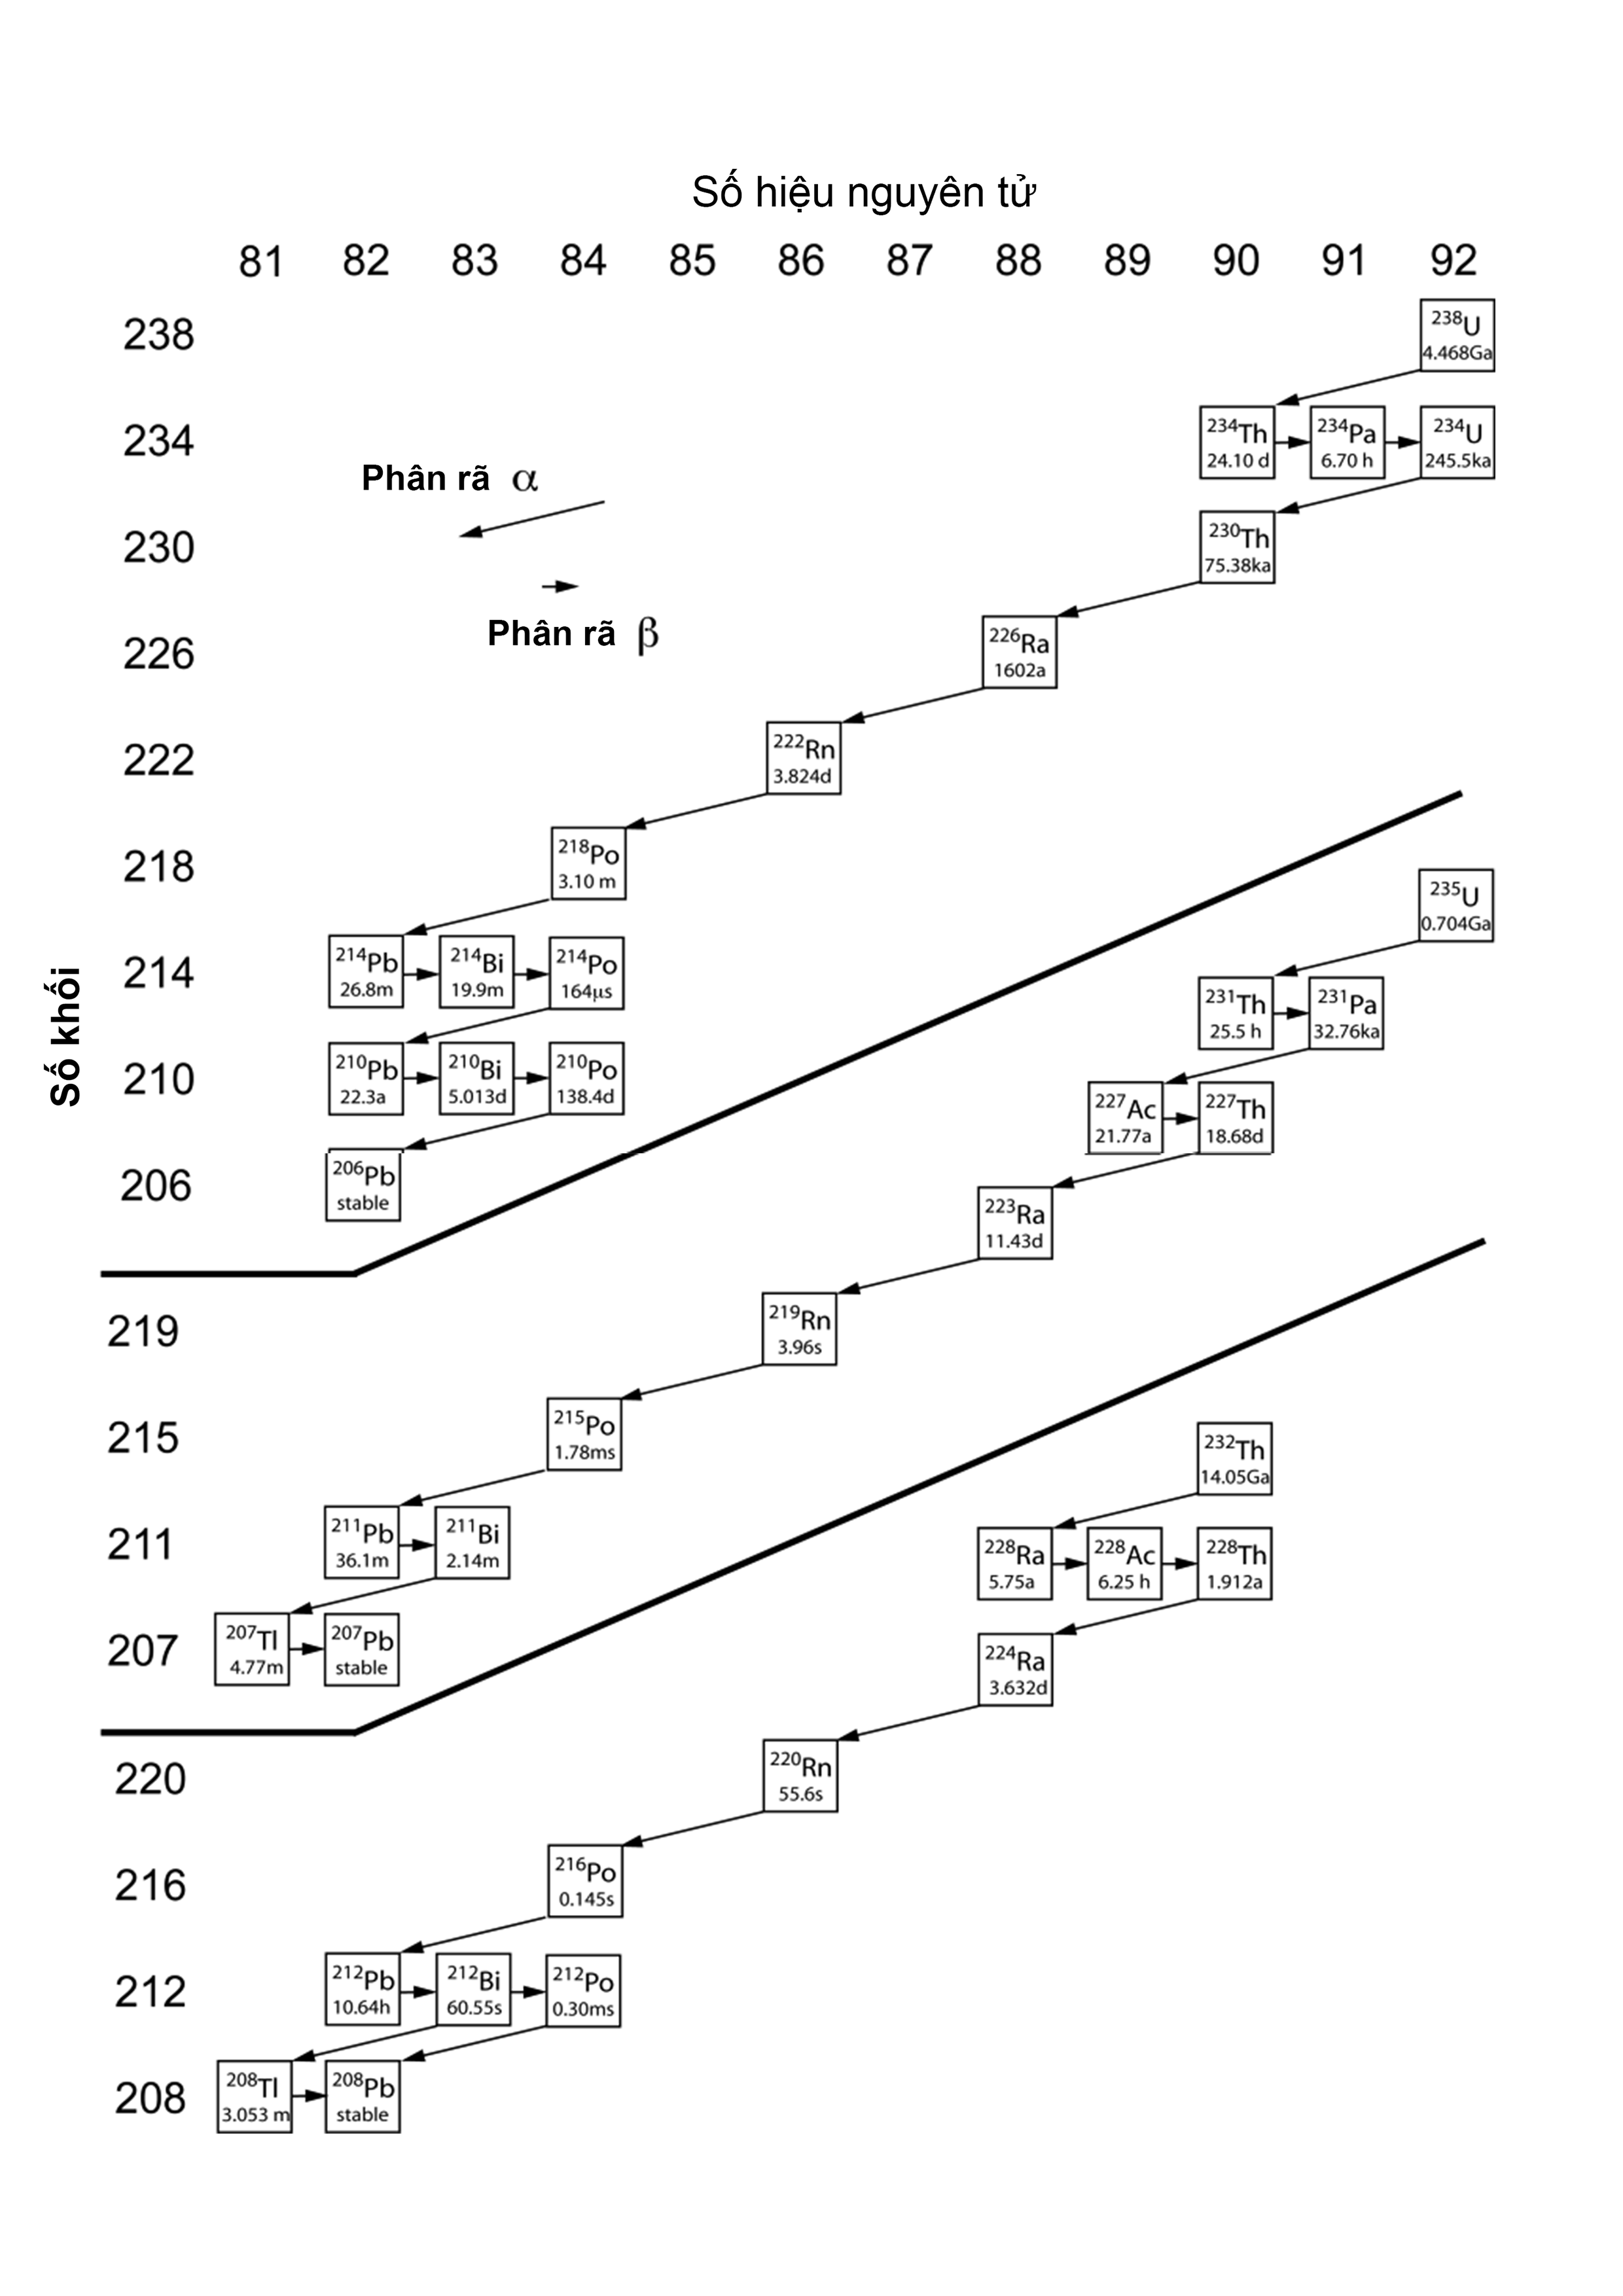
\includegraphics[width=\textwidth]{Image/Chapter1-ChainDacay.png}}
    \caption{Sơ đồ của ba chuỗi phân rã phân rã tự nhiên ~\cite{IAEANo476:revise}}
    \label{figure:ChainDecay}
\end{figure}
 

Các đồng vị của radium thường sử dụng làm chất đánh dấu trong các nghiên cứu liên quan đến địa chất, thủy văn . \ce{^223Ra} có chu kì phân rã dài nhất (1600 năm), độ phộ cập trên 99\%, phát cả bức xạ alpha và gamma trong quá trình phân rã nên được xem là đồng vị phóng xạ tự nhiên nguy hiểm nhất đối với con người và môi trường ~\cite{IAEANo476:revise}.

\begin{table}[htbp]
    \centering
    \caption{Các đồng vị của Ra trong tự nhiên ~\cite{IAEANo476:revise}}
    \label{table:RaDecay}
        \begin{tabular*}{\textwidth}{@{\extracolsep{\fill}}  *{5}{c}}
            \toprule
            Đồng vị  & Thời gian bán rã & Loại phân rã,E(MeV) & Hoạt độ riêng (Bq/g) & Đồng vị con \\
            \midrule
        \multirow{4}{*}{\ce{^223Ra}} & \multirow{4}{*}{11,43 ngày } & $\alpha_3; 5,745(9,1\%)$ & \multirow{4}{*}{$1,896 \times 10^{15}$} &   \multirow{4}{*}{\ce{^219Rn}}  \\
                            &                       & $\alpha_4; 5,714(53,7\%)$ &   & \\ 
                            &                       & $\alpha_5; 5,605(26,0\%)$ &   & \\ 
                            &                       & $\alpha_6; 5,538(9,1\%)$  &   & \\ 
        \midrule
        \multirow{2}{*}{\ce{^224Ra}} & \multirow{2}{*}{ 3,632 ngày } & $\alpha_0; 5,685(94,9\%)$ & \multirow{2}{*}{$5,92 \times 10^{15}$}  & \multirow{2}{*}{\ce{^220Rn}}\\
                            &                       & $\alpha_1; 5,685(5,1\%)$& &\\ 
        \midrule
        \multirow{2}{*}{\ce{^226Ra}} & \multirow{2}{*}{ 1600 năm } & $\alpha_0; 4,784(94,55\%)$ & \multirow{2}{*}{$3,66$}  & \multirow{2}{*}{\ce{^222Rn}} \\
                            &                       & $\alpha_1; 4,601(5,45\%)$& \\ 
        \midrule
        \ce{^228Ra}         &         5,75 năm &      $\beta; 0,046$      & $1,0 \times 10^{13}$ & \ce{^228Ac}   \\
        \bottomrule
        \end{tabular*}
\end{table}
\newpage
\section{Tính chất vật lí và hóa học của radium}

    Radium là kim loại phóng xạ thuộc nhóm IIA trong bảng tuần hoàn nguyên tố hóa học, kí hiệu Ra, số hiệu Z=88, cấu hình electron $[Rn]7s^2$, nhiệt độ nóng chảy là 973K. Radium có màu trắng xám, là kim loại mềm. Radium tinh khiết được điều chế bằng phương pháp điện phân nóng chảy \ce{RaCl2} ~\cite{Online:RadiumProperties}.

    Radium hóa đen trong không khí do bị oxi hóa tạo thành oxit RaO. Kim loại và các muối của của radium đều là các chất phát quang. Tính chất hóa học của radium tương tự các kim loại kiềm thổ khác trong nhóm như barium và canxi. Trong các phản ứng trao đổi ion, radium thường tồn tại dạng \ce{Ra^{2+}}. Bên cạnh đó, radium trong nước dễ dàng tạo phức đồng kết tủa với barit (BaSO4). Vì vậy, phương pháp đồng kết tủa BaSO4 thường được áp dụng để tách và cô lập radium trong nước  ~\cite{MnO2:RMRAlmeida}

    Radium phản ứng mạnh với các axit vô cơ như \ce{HCl}, \ce{HNO3} tạo thành các muối tan. Độ tan các muối radium được thể hiện trong bảng ~\ref{table:RaDoTan}. Các muối sulphate, carbonate, và phosphate của radium thường ít tan hơn so với muối chloride và nitrate của nó. 
    
    Radium hydroxide (\ce{Ra(OH)2}) là base có khả năng tan hơn nhiều so với các base hydroxide kiềm thổ khác. \ce{Ra(OH)2} trong dung dịch có thể dễ dàng được tách ra bằng cách thêm dung dịch ammonia \ce{NH3}H3 để hình thành phức kết tủa ~\cite{IAEANo310:revise}.

    
\begin{table}[htbp]
    \centering
    \caption{Độ tan của muối radium ở nhiệt độ $20^\circ C$ ~\cite[tr.31]{IAEANo476:revise}}
    \label{table:RaDoTan}
    \begin{tabular}{cc} 
        \hline
        Muối            &       Độ tan (g/100g \ce{H2O}) \\
        \hline
        \ce{RaCl2}      &       24,5\\
        \ce{RaBr2}      &       70,6\\
        \ce{Ra(NO3)2}   &       13,9\\
        \hline
    \end{tabular}
\end{table}




\section{Phân bố radium trong tự nhiên }

Radium phân bố trong tự nhiên (không khí, đất và nước) thông quá các quá trình hóa-lí phức tạp. Qua các tác nhân của tự nhiên và con người, radium có thể phân bố trong đất đá, khoảng sản, nước, khí quyển. Radium cũng tồn tại một phần trong cơ thể động-thực vật và con người thông qua các chuỗi thức ăn và trao đổi chất với môi trường. Hình ~\ref{figure:RadiumToBiota} thể hiện các phương thức phán tán radium trong môi trường ~\cite{IAEANo476:revise}. 


\begin{figure}[htbp]
    \centering
    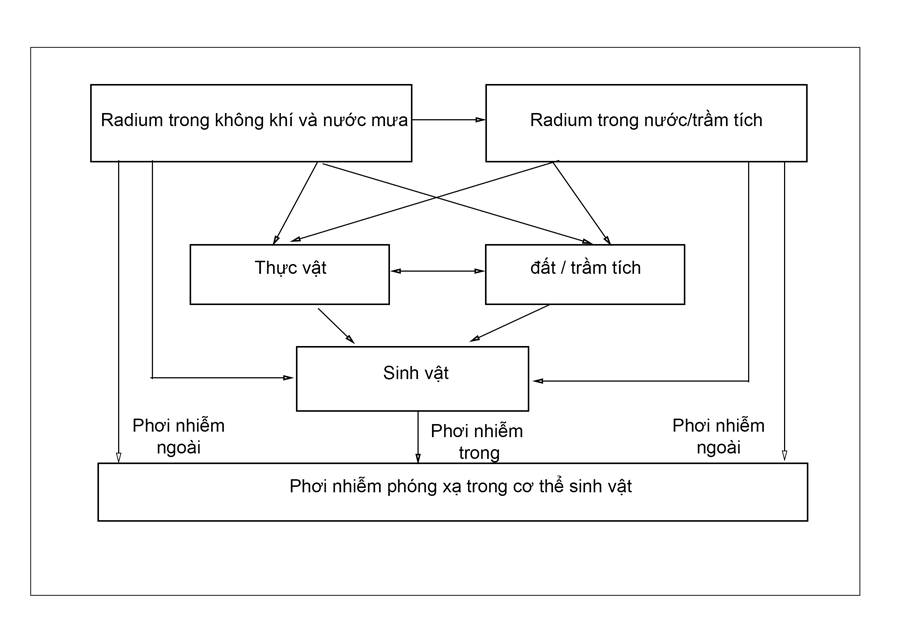
\includegraphics[width=0.95\textwidth]{Image/RadiumInBiota.png}
    \caption{Mô hình phát tán radium trong tự nhiên ~\cite{IAEANo476:revise}}
    \label{figure:RadiumToBiota}
\end{figure}
% TODO: --------------- Doc them tai lieu LAEA 410 -> Bo sung y nghia cua hinh RadiumToBioTa


   \subsection{Phân bố radium trong đất}

   Đất được hình thành từ quá trình phong hóa của đá mẹ dưới tác động của các yếu tố tự nhiên như: sự thay đổi nhiệt độ, độ ẩm, tác động của thời tiết, biến đổi khí hậu, tác động sinh học của động thực vật và con người. Do đó, các loại đất thường khác nhau về thuộc tính tùy thuộc vào đặc trưng của đá mẹ và các tác nhân ảnh hưởng từ tự nhiên. Trong quá trình phong hóa đá mẹ hình thành đất, radium được phân bố lại từ đá sang đất. Sự di chuyển của radium trong hạt đất chịu tác động rất nhiều bởi các yếu tố tự nhiên. Một phần radium được hòa tan trong nước ngầm, nước suối. Thông qua các chuỗi thức ăn, radium có thể tồn tại trong động thực vật. Phần còn lại bị lắng đọng dưới dạng phù sa, hoàng thổ hoặc hấp thụ trong đá hoặc đất ~\cite{IAEANo310:revise}. 

   Radium trong đất thể hiện các đặc điểm hóa học của một kim loại kiềm thổ. Radium hoạt động hóa học mạnh, ái lực cao. Các phản ứng trao đổi ion trong đất đóng vai trò quan trọng, ảnh hưởng đến quá trình di chuyển radium. Mỗi loại đất có các đặc tính khác nhau, khả năng trao đổi ion của các muối radium trong mỗi loại đất cũng khác nhau. Điều này ảnh hưởng đáng kể đến phân bố hàm lượng radium trong đất. Bảng ~\ref{table:RaDifferentofSoil} thể hiện hàm lượng \ce{^223Ra} trong một số loại đất khác nhau. Theo đó, hàm lượng \ce{^223Ra} trong đất dao động từ 3,7 đến 125,8 (Bq/kg). Đáng chú ý là đất nâu sa mạc ở CHLB Nga là loại đất có hàm lượng \ce{^226Ra} khá cao, từ 70,3 đến 125,8 (Bq/kg) \cite{IAEANo310:revise}.   
   
   \begin{table}[htbp]
        \centering
       \caption{Hàm lượng \ce{^226Ra} trong một số loại đất khác nhau ~\cite{IAEANo310:revise}}
       \begin{tabular}{ccc}
            \toprule
            Loại đất    &   Địa điểm    &   Hàm lượng \ce{^226Ra} (Bq/kg) \\
            \midrule
            Đất sét đỏ  & Florida, Hoa Kì  &   7,4\\
            Đất cát  &  Tây Ban Nha &  14,0 \\
            Đất Podzol  & CHLB Nga  & 33,3  \\
            Đất rừng xám  & CHLB Nga  & 37,1  \\
            Đất sét đen  & CHLB Nga  & 29,6  \\
            Đất rừng nâu  & CHLB Nga  & 29,6  \\
            Đất đỏ  & CHLB Nga  & 40,7  \\
            Đất xám/đất sa mạc  & CHLB Nga  & 18,5 \\
            Đất nâu sa mạc   & CHLB Nga  & 70,3 - 126  \\
            \bottomrule
        \end{tabular}
       \label{table:RaDifferentofSoil}
   \end{table}
   
        Bảng ~\ref{table:RaDifferentofCountry} thể hiện hàm lượng \ce{^226Ra} trong đất ở một số quốc gia khác nhau. Hàm lượng 226Ra nằm trong khoảng 2,59 - 140,6 (Bq/kg) đối với tất cả các quốc gia này.  ~\cite{IAEANo310:revise}.

    \begin{table}[htbp]
        \centering
        \caption{Hàm lượng \ce{^226Ra} trong đất ở một số quốc gia ~\cite{IAEANo310:revise}}
        \begin{tabular}{cc}
            \toprule
            Quốc gia   &   Hàm lượng \ce{^226Ra}  (Bq/kg)\\
            \midrule
            Tiệp Khắc   & 3,7 - 141\\
           Đức          & 13,0 - 48,1\\
            Ireland     & 48,1 - 107\\
            Anh         & 2,96 - 55,5\\
            CHLB Nga    & 3,7 - 48,1 \\
            Phần Lan    & 37 - 51,8\\
            Hoa Kì      & 29,6 - 104\\
            Nam Tư      & 29,4 - 37,4\\
            Nhật Bản    &  5,55 - 38,9\\
            Ấn Độ       & 2,59 - 26,3\\

            \bottomrule
        \end{tabular}
        \label{table:RaDifferentofCountry}
    \end{table}
 
    Bảng ~\ref{table:RaHighConcentration} thể hiện một số khu vực có hàm lượng \ce{^226Ra} cao nhất trên thế giới. Giá trị cao nhất đo được tại các vùng Ramsar, Iran và Cộng hòa Komi, CHLB Nga, vượt va so với hàm lượng \ce{^226Ra} trung bình trong đất trên thế giới theo tiêu chuẩn UNSCEAR  ~\cite{IAEANo476:revise}. 
    
    \begin{table}[htbp]
        \centering
        \caption{Hàm lượng \ce{^226Ra} trong đất ở một số khu vực cao nhất thế giới ~\cite{IAEANo476:revise}}
        \begin{tabular}{cc}
            \toprule
            Quốc gia    & Hàm lượng \ce{^226Ra} (Bq/kg) \\
            \midrule
            Kerala, Ấn Độ & 7,8-1520 \\
            Araxa, Brazil &  703-42400 \\
            Tapira, Brazil &  7814-28 800 \\
            Núi Ambazac Pháp &  950-8860 \\
            Ramsar, Iran  & 740-37 000 \\
            Niue, New Zealand & 6920-12 400 \\
            \bottomrule
        \end{tabular}
        \label{table:RaHighConcentration}
    \end{table}

    \subsection{Phân bố radium trong nước ngầm }
    

Radium trong nước ngầm là kết quả tương tác của dòng chảy mạch nước ngầm qua bề mặt, khe nứt của đá,... Các tương tác này tạo điều kiện cho radium sinh ra từ đồng vị mẹ dễ dàng hoà tan vào nước. Hàm lượng phóng xạ radium trong nước còn phụ thuộc mạnh vào các đặc điểm địa chất, độ sâu mực nước, độ pH, tốc độ dòng chảy, nhiệt độ môi trường nước, thời điểm lấy nước, và lượng mưa. Bên cạnh đó, các quá trình khai thác nhiên liệu, khai thác quặng uranium để sản xuất nguyên liệu hạt nhân, khai thác quặng photphat - apatit để sản xuất phân lân, vàng, than đá, ... cũng góp phần làm tăng đáng kể hàm lượng phóng xạ radium trong nước.

Với đặc tính dễ hòa tan của muối radium và tạo phức kết tủa với muối sulphat của barium va canxi, qua các khe nứt của thành đá gây ra bởi các hoạt động khai thác của con người, radium dễ dàng có mặt trong mạch nước. Quá trình khai thác dầu khí tạo ra một lượng lớn bùn thải. Việc xử lí bùn thải do khai thác dầu khí thường rất tốn kém nên đa phần được chôn lấp. Điều này dẫn đến nhiều rủi ro ô nhiễm phóng xạ, đặc biệt là mạch nước ngầm tại các khu vực dễ tiếp xúc với bùn thải ~\cite{IAEANo476:revise}.
 

Nồng độ \ce{^226Ra} trong nước ngầm tại một số khu vực trên thế giới được thể hiện trong bảng ~\ref{table:RadiumInGroundWater}. Theo đó, \ce{^226Ra} có nồng độ khá cao trong một số loại nước ở các khu vực khác nhau như khoáng nóng tại Nhật Bản (1300-7840 mBq/L), nước ngầm tại vùng khai thác uranium ở Texas - Hoa Kì (14,8-6290 mBq/L), nước nóng của địa nhiệt tại miền Tây - Hoa Kì (1,52-55 500) ~\cite{IAEANo476:revise}.

\begin{table}[htbp]
    \centering
    \caption{Nồng độ \ce{^226Ra} trong nước ngầm ở một số khu vực ~\cite{IAEANo476:revise}}
    \begin{tabular}{c c >{\centering\arraybackslash}m{3.7cm} c }
        \toprule
        Địa điểm    &   Nguồn nước &    Mô tả   & Nồng độ \ce{^226Ra} (mBq/L)\\
        \midrule
        Salzburg, Áo & Nước giếng &  & <3,7-270 \\
        Helsinki, Phần Lan & Nước giếng khoan &  & <3,7-9470 \\
      Pháp & Nước suối khoáng &  &163 \\
        Anh  & Nước khoáng nóng &  &374-525 \\
        \midrule
        Nhật Bản & Nước khoáng nóng  &  & 1300-7840\\
        Ả Rập Xê Út & Nước suối  &  & 699\\
        Đài Loan & Nước khoáng nóng  &  & 1,85-588\\
        \midrule
        Ottawa,Hoa Kì & Nước giếng & Nước đã lọc tại nhà máy & 3,7-570 \\
        Illinois,Hoa Kì & Nước giếng & Nước chưa qua xử lí & 0,74-836 \\
        Ottawa,Hoa Kì & Nước giếng & Nước đã lọc tại nhà máy & 3,7-570 \\
        Grants,Hoa Kì & Nước ngầm & Nhà máy khai thác quặng uranium & 1,9-1960 \\
        Texas,Hoa Kì & Nước ngầm & Nhà máy khai thác và nghiền quặng uranium & 14,8-6290 \\
        Florida,Hoa Kì & Nước ngầm & Nhà máy khai thác quặng photphat & 2810 \\
        Miền Tây, Hoa Kì & Nước nóng của địa nhiệt & Rò rĩ nguồn nước địa nhiệt & 1,52 - 55 550 \\
        \midrule 
        Yeelirrie, Úc & Nước ngầm & Mỏ quặng uranium & 18,5-33 400 \\
        \bottomrule
    \end{tabular}
    \label{table:RadiumInGroundWater}
\end{table}



\subsection{Phân bố radium trong không khí }

Bên cạnh tập trung trong đất và nước ngầm, một phần radium cũng tồn tại trong các hạt bụi khí nhỏ. Nồng độ \ce{^226Ra} trung bình trong bụi khí trên thế giới khoảng $1,5\mu Bq/m^3$ ~\cite{IAEANo476:revise}. Các hoạt động khai thác nhiên liệu của con người góp phần làm tăng nồng độ radium trong bụi khí. Đặc biệt, trong đó, ngành công nghiệp nhiệt điện là một trong những ngành làm tăng đáng kể nồng độ radium trong không khí. Trong quá trình đốt than, nhiệt độ lên đến $1700 ^\circ C$, than được nung nóng chảy thành tro. Tro bay cùng với hơi nước được thải ra ngoài khí quyển, đóng góp đáng kể vào lượng radium trong không khí. Bên cạnh đó, lượng tro bay này có thể lắng đọng xuống mặt đất, thảm thực vật hoặc nước mặt và thậm chí có thể xâm nhập vào nước ngầm.
            
\section{Ảnh hưởng của radium đến sức khỏe con người}

Thông qua nhiều chuỗi chuyển hóa sinh - hóa và chuỗi thức ăn mà radium có thể tồn tại trong cơ thể con người và sinh vật. Hình ~\ref{figure:RadiumToHuman} thể hiện tóm quá trình chuyển hóa radium từ môi trường tự nhiên vào cơ thể con người. Quá trình này diễn ra phức tạp và chịu ảnh hưởng bởi nhiều yếu tố trong môi trường và sinh vật. Về cơ bản, radium từ môi trường đi vào cơ thể con người chủ yếu qua đường hô hấp và tiêu hóa ~\cite{IAEANo476:revise}.

Trong cơ thể con người, radium phân rã alpha, hình thành các đồng vị con cháu phân rã alpha, beta hoặc gamma \cite{IAEANo310:revise}. Đồng vị \ce{^226Ra} là đồng vị phóng xạ nguy hiểm hơn cả do chu kỳ bán rã lớn, xác suất phát alpha cao, năng lượng phân rã lớn. Trong cơ thể con người, \ce{^226Ra} chủ yếu tích tụ trong xương, răng. Với khoảng 2,5 mg \ce{^226Ra} trong cơ thể, con người sẽ nhận một liều chiếu khoảng 25 Sv. Các bệnh thường gây ra khi chủ yếu tập trung ở xương, rrangnhư ung thư xương, thoái hóa xương, răng,...~\cite{Thesis:HNPThu}.

   \begin{figure}[htbp]
    \centering
    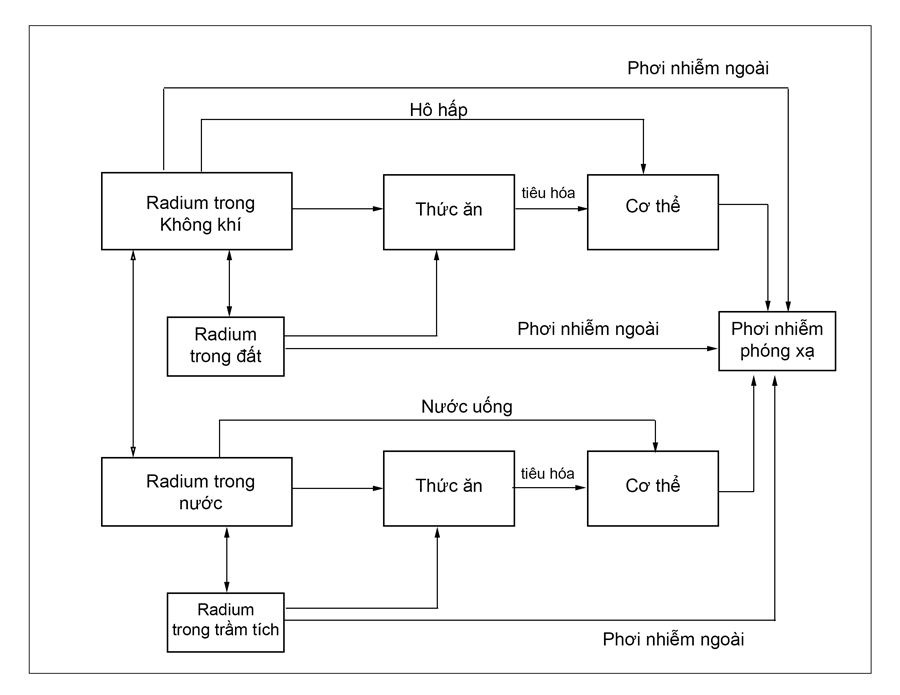
\includegraphics[width=0.75\textwidth]{Image/RadiumInHuman.png}
    \caption{Sơ đồ các con đường di chuyển của radium từ môi trường vào cơ thể người ~\cite{IAEANo476:revise}}
    \label{figure:RadiumToHuman}
\end{figure}
      
\clearpage



% ----------- Track Changes 
% REVIEW: 2019.01.06 - 11.51PM: Completed